\section{Introduction}
\label{sec:intro}

Linguistic expressions are coreferent if they refer to the same
entity.
The computational task of discovering coreferent mentions is coreference
resolution (\coref).
Neural models~\citep{lee-2018,joshi-2020} are \abr{sota}
on \ontonotes~{\small 5.0}~\citep{pradhan-2013} but
cannot immediately generalize to other datasets.
Generalization is difficult because domains differ in content, writing style, and annotation
guidelines.
To overcome these challenges, models need copiously labeled,
in-domain data~\citep{bamman-2020}.

Despite expensive labeling costs, adapting \coref{} is crucial for applications like
uncovering information about proteins in biomedicine~\citep{kim-2012}
and distinguishing entities in legal documents~\citep{gupta-2018}.
Ideally, we would like to quickly and cheaply adapt the model without repeatedly relying on an excessive amount of annotations to retrain the model.
To reduce labeling cost, we investigate active learning~\citep{settles-2009}
for \coref{}.  Active learning aims to reduce annotation costs by
intelligently selecting examples to label.
Prior approaches use active learning to improve the model within the same domain~\citep{gasperin-2009,sachan-2015} without considering adapting to new data distributions.
For domain adaptation in \coref{},
\citet{zhao-2014} motivate the use of active learning
to select out-of-distribution examples.
A word like ``the bonds'' refers to municipal bonds in
\ontonotes{} but links to ``chemical bonds'' in another
domain (Figure~\ref{fig:example}).
If users annotate the antecedents of ``the
bonds'' and other ambiguous entity mentions, then these labels
help adapt a model trained on \ontonotes{} to new domains.

Active learning for \coref{} adaptation is well-motivated, but the implementation is neither straightforward nor well-studied.
First, \coref{} is a span detection and clustering task,
so selecting which spans to label is more complicated than
choosing independent examples for text classification.
Second, \coref{} labeling involves closely reading the
documents.
Labeling more spans within the same context is more efficient.  However, labeling more spans across different documents increases data diversity and may
improve model transfer.
How should we balance these competing objectives?

\begin{figure*}
    \center
    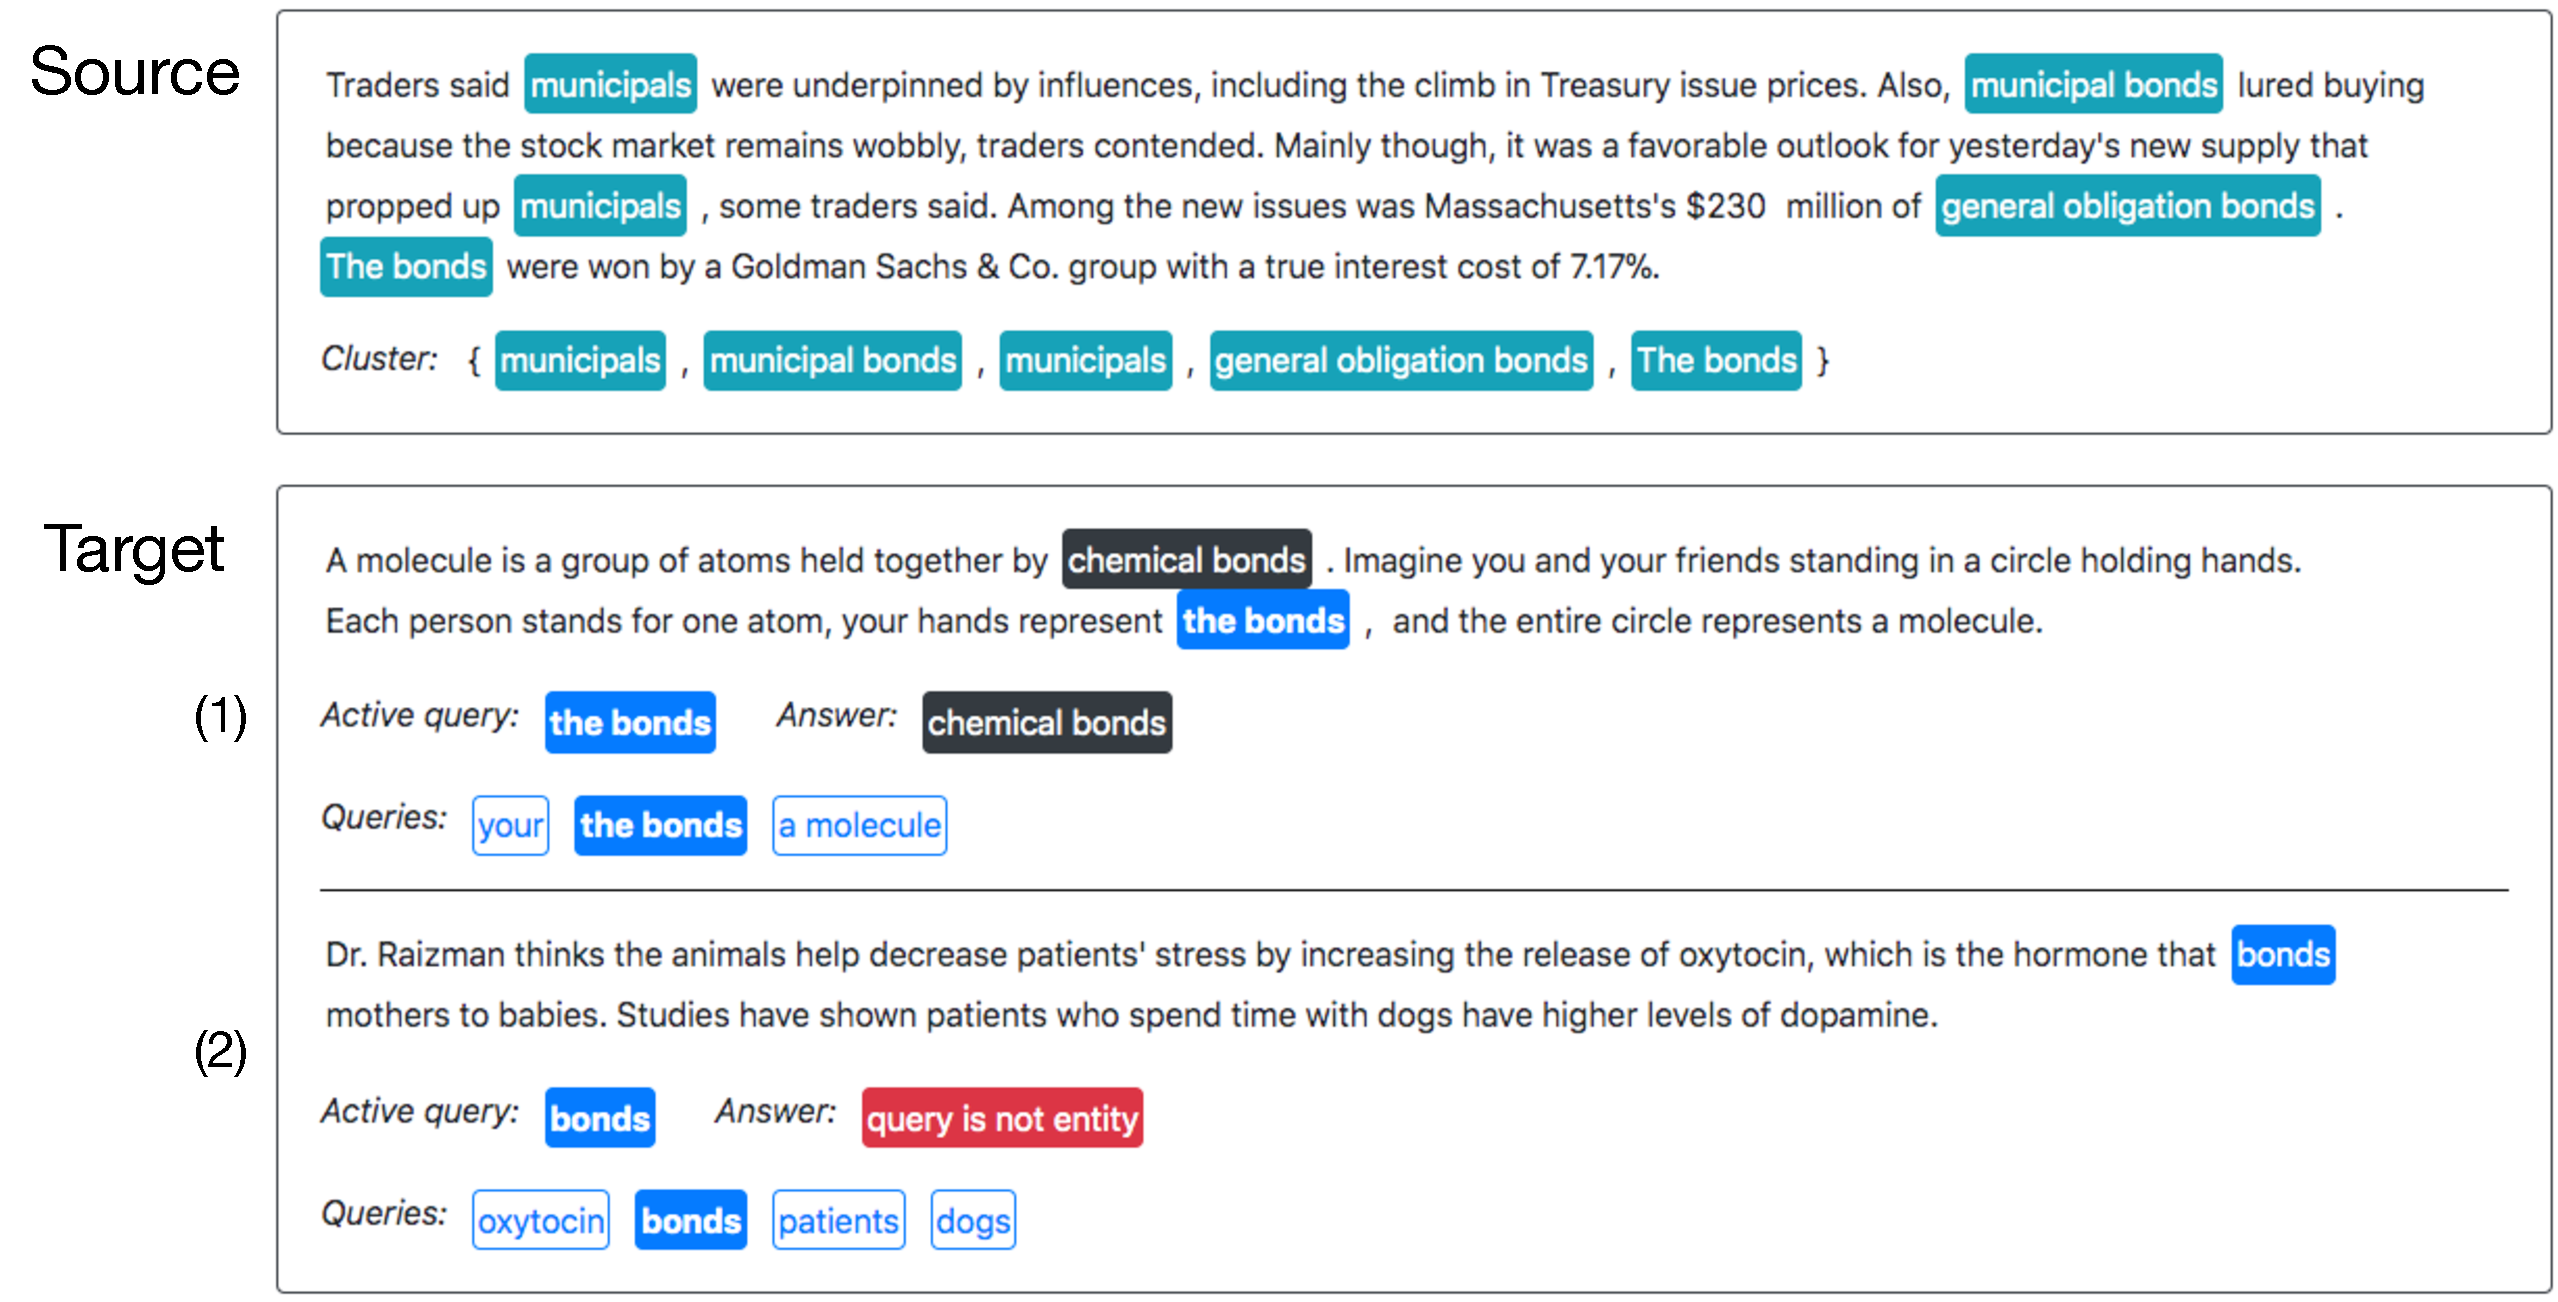
\includegraphics[width=\linewidth]{example.pdf}
    \caption{
        \coref{} models are trained on \textbf{source} domain \ontonotes{}, which contains data like
        news articles. The \textbf{source}
        document links ``the bonds'' to ``municipal bonds''.
        In a \textbf{target} domain like \preco{}~\citep{chen-2018-preco}, ``the bonds'' may no longer
        have the same meaning. It can refer to
        ``chemical bonds'' (Document 1) or not be considered an entity (Document 2).
        A solution is to continue training the \textbf{source} model on more spans
        from the \textbf{target} domain. Active learning helps select
        ambiguous spans, like ``the bonds'', for the user to label on this interface (Section~\ref{ssec:human_labeling}).
    }
    \label{fig:example}
  \end{figure*}


Our paper extends prior work in active
learning for \coref{} to the problem of coreference model
transfer~\citep{xia-2021}:
\begin{enumerate*}
    \item We generalize the \emph{clustered entropy} sampling
        strategy~\citep{li-2020} to include uncertainty in mention detection. We analyze the effect of
        each strategy on coreference model transfer.
    \item We investigate the trade-off between labeling and reading
    through simulations and a real-time user study.
    Limiting annotations to the same document
    increases labeling throughput and decreases volatility in model
    training.
\end{enumerate*}
Taken together, these contributions offer a blueprint for faster creation of \coref{} models
across domains.\footnote{\url{https://github.com/forest-snow/incremental-coref}}

